A graph in it's simplest form is an ordered triple consisting of a nonempty set of vertices, a set of edges which are disjoint from the set of vertices and an incident function which associates each edge with an unordered pair of vertices \cite{bondy1976graph}. As an example, let us consider the graph $G$ shown in Fig. \ref{fig:Simple_graph}. $V(G)$ is the set of vertices and $E(G)$ is the set of edges and $\psi_G$ is the incident function. The graph visualized in the figure can be represented using (\ref{eq:GRAPH1}).\\

\begin{figure}[!htb]
\centering
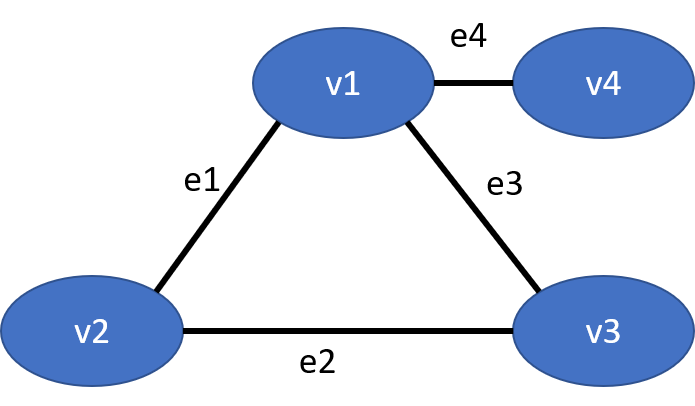
\includegraphics[width=0.5\linewidth]{figs/A8/Simple_graph.png}
\caption{Visual representation of graph G}
\label{fig:Simple_graph}
\vspace{-3mm}
\end{figure}

\begin{equation}
\label{eq:GRAPH1}
   G = (V(G), E(G), \psi_G)
\end{equation}
where,
$$
V(G) = \{v1,v2,v3,v4\} 
$$
$$
E(G) = \{e1, e2, e3, e4\}
$$
and $\psi_G$ is defined by 

\begin{equation*}
\begin{tabular}{lllll}
$\psi_G(e1) = v1,v2$, &$\psi_G(e2) = v2,v3$,  &$\psi_G(e3) = v2,v3$ & and & $\psi_G(e4) = v1,v4$
\end{tabular}
\end{equation*}

In this case, it should be noted that the pairs used in $\psi_G$ are unordered. $\psi_G(e1)$ can be represented as v1,v2 or v2,v1. This form of a graph is called an undirected simple graph. 

A graph that uses an ordered pair to define edges is called a directed graph. The formal definition of a directed graph is defined as an ordered pair $D = (V,A)$ \cite{bang2008digraphs}. $V$ is a nonempty set of vertices or nodes and $A$ is a set of ordered pairs of vertices known as edges. Fig. \ref{fig:D_graph} shows a directed graph representation of the graph shown in Fig. \ref{fig:Simple_graph}. The mathematical representation of the graph is as follows. The graph shown in Fig. \ref{fig:D_graph} is named $H$. The mathematical representation of $H$ is shown in (\ref{eq:GRAPH2}).

\begin{figure}[!htb]
\centering
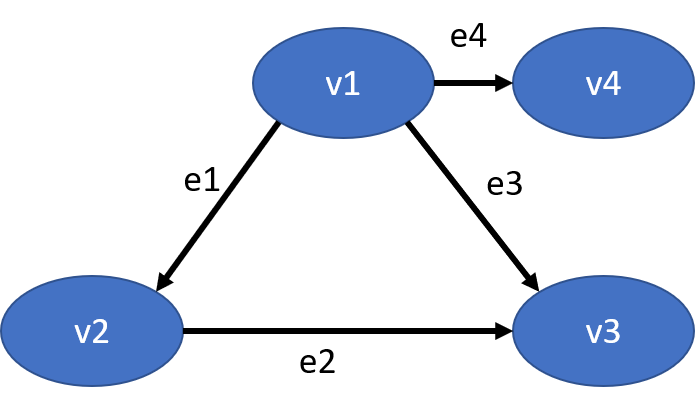
\includegraphics[width=0.5\linewidth]{figs/A8/D_graph.png}
\caption{Visual representation of a directed graph H.}
\label{fig:D_graph}
\vspace{-3mm}
\end{figure}

\begin{equation}
\label{eq:GRAPH2}
   H = (V(H), A(H))
\end{equation}
where,
$$
V(H) = \{v1,v2,v3,v4\} 
$$
$$
A(H) = \{(v1,v2), (v2,v3), (v1,v3), (v1,v4)\}
$$

It should be noted that the elements of $A(H)$ are ordered. The next section formulates the energy management problem as a directional graph.